\documentclass[12pt, a4paper, oneside]{article}\usepackage{graphicx, color}
%% maxwidth is the original width if it is less than linewidth
%% otherwise use linewidth (to make sure the graphics do not exceed the margin)
\makeatletter
\def\maxwidth{ %
  \ifdim\Gin@nat@width>\linewidth
    \linewidth
  \else
    \Gin@nat@width
  \fi
}
\makeatother

\definecolor{fgcolor}{rgb}{0.2, 0.2, 0.2}
\newcommand{\hlnumber}[1]{\textcolor[rgb]{0,0,0}{#1}}%
\newcommand{\hlfunctioncall}[1]{\textcolor[rgb]{0.501960784313725,0,0.329411764705882}{\textbf{#1}}}%
\newcommand{\hlstring}[1]{\textcolor[rgb]{0.6,0.6,1}{#1}}%
\newcommand{\hlkeyword}[1]{\textcolor[rgb]{0,0,0}{\textbf{#1}}}%
\newcommand{\hlargument}[1]{\textcolor[rgb]{0.690196078431373,0.250980392156863,0.0196078431372549}{#1}}%
\newcommand{\hlcomment}[1]{\textcolor[rgb]{0.180392156862745,0.6,0.341176470588235}{#1}}%
\newcommand{\hlroxygencomment}[1]{\textcolor[rgb]{0.43921568627451,0.47843137254902,0.701960784313725}{#1}}%
\newcommand{\hlformalargs}[1]{\textcolor[rgb]{0.690196078431373,0.250980392156863,0.0196078431372549}{#1}}%
\newcommand{\hleqformalargs}[1]{\textcolor[rgb]{0.690196078431373,0.250980392156863,0.0196078431372549}{#1}}%
\newcommand{\hlassignement}[1]{\textcolor[rgb]{0,0,0}{\textbf{#1}}}%
\newcommand{\hlpackage}[1]{\textcolor[rgb]{0.588235294117647,0.709803921568627,0.145098039215686}{#1}}%
\newcommand{\hlslot}[1]{\textit{#1}}%
\newcommand{\hlsymbol}[1]{\textcolor[rgb]{0,0,0}{#1}}%
\newcommand{\hlprompt}[1]{\textcolor[rgb]{0.2,0.2,0.2}{#1}}%

\usepackage{framed}
\makeatletter
\newenvironment{kframe}{%
 \def\at@end@of@kframe{}%
 \ifinner\ifhmode%
  \def\at@end@of@kframe{\end{minipage}}%
  \begin{minipage}{\columnwidth}%
 \fi\fi%
 \def\FrameCommand##1{\hskip\@totalleftmargin \hskip-\fboxsep
 \colorbox{shadecolor}{##1}\hskip-\fboxsep
     % There is no \\@totalrightmargin, so:
     \hskip-\linewidth \hskip-\@totalleftmargin \hskip\columnwidth}%
 \MakeFramed {\advance\hsize-\width
   \@totalleftmargin\z@ \linewidth\hsize
   \@setminipage}}%
 {\par\unskip\endMakeFramed%
 \at@end@of@kframe}
\makeatother

\definecolor{shadecolor}{rgb}{.97, .97, .97}
\definecolor{messagecolor}{rgb}{0, 0, 0}
\definecolor{warningcolor}{rgb}{1, 0, 1}
\definecolor{errorcolor}{rgb}{1, 0, 0}
\newenvironment{knitrout}{}{} % an empty environment to be redefined in TeX

\usepackage{alltt} % Paper size, default font size and one-sided paper
%\graphicspath{{./Figures/}} % Specifies the directory where pictures are stored
%\usepackage[dcucite]{harvard}
\usepackage{rotating}
\usepackage{amsmath}
\usepackage{setspace}
\usepackage{pdflscape}
\usepackage[flushleft]{threeparttable}
\usepackage{multirow}
\usepackage[comma, sort&compress]{natbib}% Use the natbib reference package - read up on this to edit the reference style; if you want text (e.g. Smith et al., 2012) for the in-text references (instead of numbers), remove 'numbers' 
\usepackage{graphicx}
%\bibliographystyle{plainnat}
\bibliographystyle{agsm}
\usepackage[colorlinks = true, citecolor = blue, linkcolor = blue]{hyperref}
%\hypersetup{urlcolor=blue, colorlinks=true} % Colors hyperlinks in blue - change to black if annoying
%\renewcommand[\harvardurl]{URL: \url}
\IfFileExists{upquote.sty}{\usepackage{upquote}}{}
\begin{document}
\title{Commodity Futures}
%\author{Rob Hayward\footnote{University of Brighton Business School, Lewes Road, Brighton, BN2 4AT; Telephone 01273 642586.  rh49@brighton.ac.uk}}
\date{\today}
\maketitle
\section*{Introduction}
Commodities are primarily traded in futures markets.  These are an agreement now to pay a particular price for a particular commodity at some set date in the future. These markets are mostly exchange traded and are therefore the quantities to be supplied and the dates at which this will be done are standardised.  Standardisation makes the contract more widely applicable and increases liquidity.  The difference between the underlying risk that is to be hedge by these contracts and the futures is called the \emph{basis risk}.  

The futures market is divided into two types of activity:  hedging and speculation.  The hedgers aim to reduce risk by locking in the price that they will buy or sell the commodity in the future.  For example, the oil hedgers will be oil companies, airline companies and other producers and users of oil and related products. The speculators taking a position in the market because they believe that they can make a profit from price movement.  Keynes and Hicks argued that futures prices would tend to trade at a discount to the spot price because speculators would require some payment for taking risk from the hedgers. 

The US Commodity and Futures Trading Commission (CFTC), a regulatory body, requires that all participants in the futures market categorise themseleves as \emph{commerical} with some underlying business interest in the 

\section*{Pricing futures contracts}
The price of a futures contract should be equal to the cost of buying the commodity now and storing it until the delivery date.  For a financial serucity where the only cost is the cost of finance, the $F(t, T)$ futures price for time $T$, valued at $t$, where $t<T$ is equal to, 
\begin{equation*}
F(t, T) = S(t) \times (1 +r)^{(T-t)}
\end{equation*}
or, in continuous time, 
\begin{equation*}
F(t, T) = S(t)e^{r(T-t)}
\end{equation*}
For other futures, storage costs, income in the form of dividends and coupons and any other benefits that accrue from the holding of the commodity. This may be particularly important if there are large storage costs involved for commoditie. 


\begin{knitrout}
\definecolor{shadecolor}{rgb}{0.969, 0.969, 0.969}\color{fgcolor}\begin{kframe}
\begin{alltt}
\hlfunctioncall{require}(xts)
\end{alltt}


{\ttfamily\noindent\itshape\color{messagecolor}{\#\# Loading required package: xts}}

{\ttfamily\noindent\color{warningcolor}{\#\# Warning: package 'xts' was built under R version 3.0.2}}

{\ttfamily\noindent\itshape\color{messagecolor}{\#\# Loading required package: zoo}}

{\ttfamily\noindent\itshape\color{messagecolor}{\#\# \\\#\# Attaching package: 'zoo'}}

{\ttfamily\noindent\itshape\color{messagecolor}{\#\# The following object is masked from 'package:base':\\\#\# \\\#\#\ \ \ \  as.Date, as.Date.numeric}}\begin{alltt}
da <- \hlfunctioncall{read.csv}(\hlstring{"http://www.quandl.com/api/v1/datasets/CFTC/CL_F_L_ALL.csv?&trim_start=2000-02-08&trim_end=2014-02-18&sort_order=desc"}, 
    colClasses = \hlfunctioncall{c}(Dates = \hlstring{"Date"}))
db <- \hlfunctioncall{read.csv}(\hlstring{"http://www.quandl.com/api/v1/datasets/OFDP/FUTURE_CL1.csv?&auth_token=mUCjthkJFQDsYVrFh4Gh&trim_start=2000-02-08&trim_end=2014-02-26&collapse=monthly&sort_order=desc"}, 
    colClasses = \hlfunctioncall{c}(Date = \hlstring{"Date"}))
da$spec <- (da[, 3] - da[, 4])/(da[, 3] + da[, 4])
da$hedge <- da[, 6] - da[, 7]
\hlfunctioncall{par}(mfrow = \hlfunctioncall{c}(2, 1))
\hlfunctioncall{plot}(da$spec ~ da$Date, type = \hlstring{"l"}, main = \hlstring{"Oil price and Spculative Positions"})
\hlfunctioncall{plot}(db$Settle ~ db$Date, type = \hlstring{"l"}, main = \hlstring{"Oil and "})
\end{alltt}
\end{kframe}
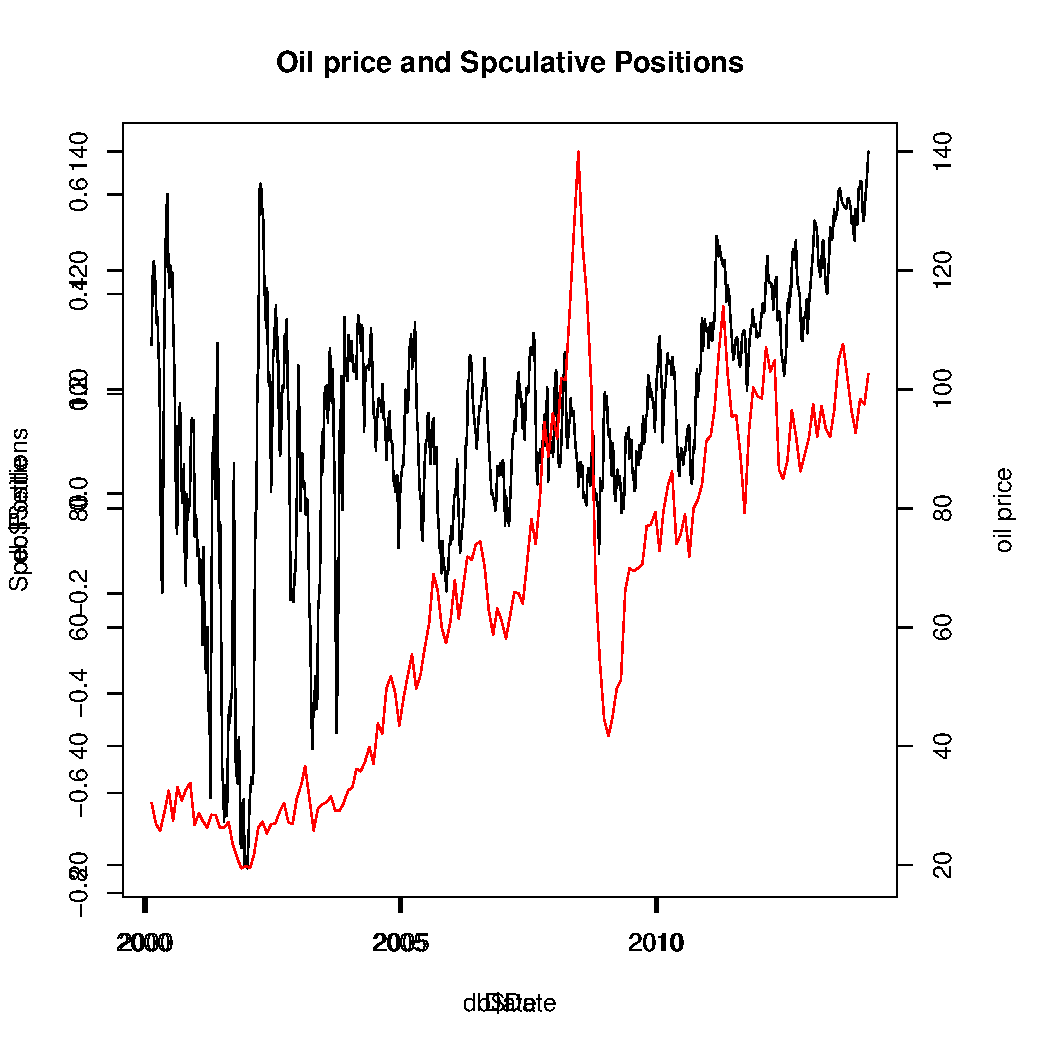
\includegraphics[width=\maxwidth]{figure/Oil} 
\begin{kframe}\begin{alltt}
\hlfunctioncall{head}(db)
\end{alltt}
\begin{verbatim}
##         Date   Open   High    Low Settle Volume Open.Interest
## 1 2014-02-28 102.04 102.90 101.58 102.59 196518        320864
## 2 2014-01-31  97.97  98.39  97.10  97.49 268687        314926
## 3 2013-12-31  99.25  99.39  98.15  98.42 127689        267603
## 4 2013-11-30  92.33  93.90  92.06  92.72 159719        341643
## 5 2013-10-31  96.62  97.03  96.03  96.38 267311        354643
## 6 2013-09-30 102.46 102.76 101.05 102.33 242415        314427
\end{verbatim}
\end{kframe}
\end{knitrout}


Delivery...

Supply and Demand

Trade the spread




\end{document}
